\subsection{Cálculo de coeficientes de pressão no cilindro}

% Anteriormente ao início da coleta de dados, verificou-se a adequada instalação do cilindro e do tubo de Pitot na câmara de ensaio, conforme determinam as boas práticas para um procedimento efetivo. O cilindro possui um orifício, no qual a tomada de pressão ao longo do experimento é realizada. Configura-se o cilindro na posição inicial correspondente a 0° (ângulo entre a direção axial do orifício e a direção vertical). 

% Os terminais de um micromanômetro foram conectados à tomada de pressão estática local e ao tubo de Pitot, para assim retornar o cálculo diferencial entre as pressões estáticas local e do escoamento livre correspondente a cada ponto de ensaio. Ligou-se então o túnel e se iniciou a coleta de valores de pressão dinâmica para valores graduais de rotação do cilindro, de 0° (valor inicial) a 180°. Considerando a simetria axial do cilindro, este conjunto de dados é suficiente para se determinar resultados para toda posição do orifício ao redor da seção transversal do objeto de ensaio. Entre 180° e 360°, a curva deve convergir e se estabilizar, pois o orifício se encontra obstruído pelo cilindro em relação à direção do escoamento.

% Seguiu-se então para o cálculo dos coeficientes de pressão a partir dos valores de pressão dinâmica coletados. Como na configuração inicial do cilindro a posição do orifício coincide com o ponto de sucção, o valor obtido pelo micromanômetro nesta medida é por definição igual à tomada de pressão dinâmica do escoamento livre. Assim, cada coeficiente de pressão se dá pela divisão entre o dado coletado no ponto em cada medida e o dado coletado no ponto inicial. 
Antes de iniciar a coleta de dados, foi verificada a instalação adequada do cilindro e do tubo de Pitot na câmara de ensaio, seguindo boas práticas. O cilindro possui um orifício para medição de pressão e é posicionado inicialmente a 0° em relação à vertical. Os terminais de um micromanômetro foram conectados para calcular a diferença entre as pressões estáticas local e do escoamento livre. Após ligar o túnel de vento, foram coletados dados de pressão dinâmica variando a rotação do cilindro de 0° a 180°. Devido à simetria axial do cilindro, esses dados são suficientes para determinar os resultados para toda a seção transversal do objeto. Entre $180^\circ$ e $360^\circ$, a curva deve convergir e estabilizar, pois o orifício fica obstruído pelo cilindro em relação ao escoamento.

Em seguida, foram calculados os coeficientes de pressão a partir dos valores de pressão dinâmica coletados. Na configuração inicial, a posição do orifício coincide com o ponto de sucção, tornando o valor obtido pelo micromanômetro igual à pressão dinâmica do escoamento livre. Cada coeficiente de pressão é obtido dividindo o dado coletado em cada medição pelo dado do ponto inicial.

\begin{figure}[htbp]
    \centering
    \begin{subfigure}{0.35\textwidth}
        \centering
        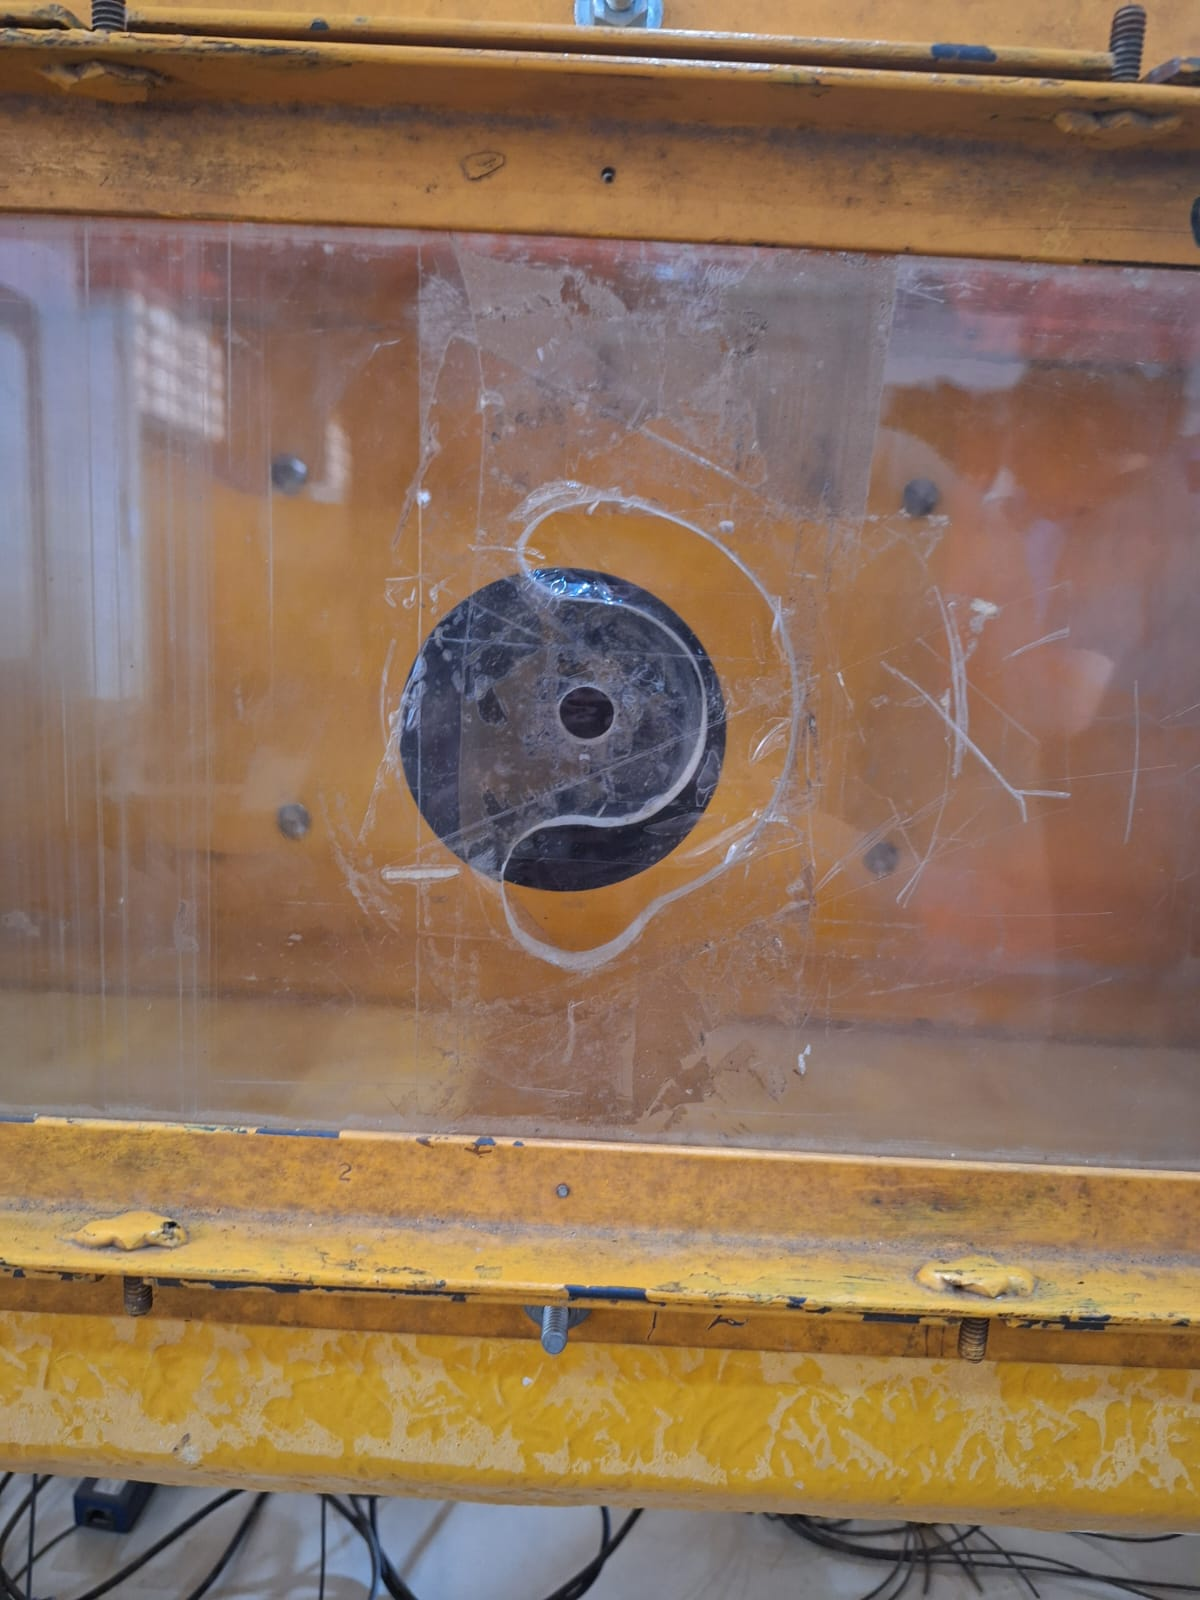
\includegraphics[width=\textwidth]{01.Parte1/Figuras/Cilindro - representação - vista da seção.jpg}
        \caption{Seção transversal do cilindro}
        \label{fig:SecTrans}
    \end{subfigure}
    \hfill
    \begin{subfigure}{0.55\textwidth}
        \centering
        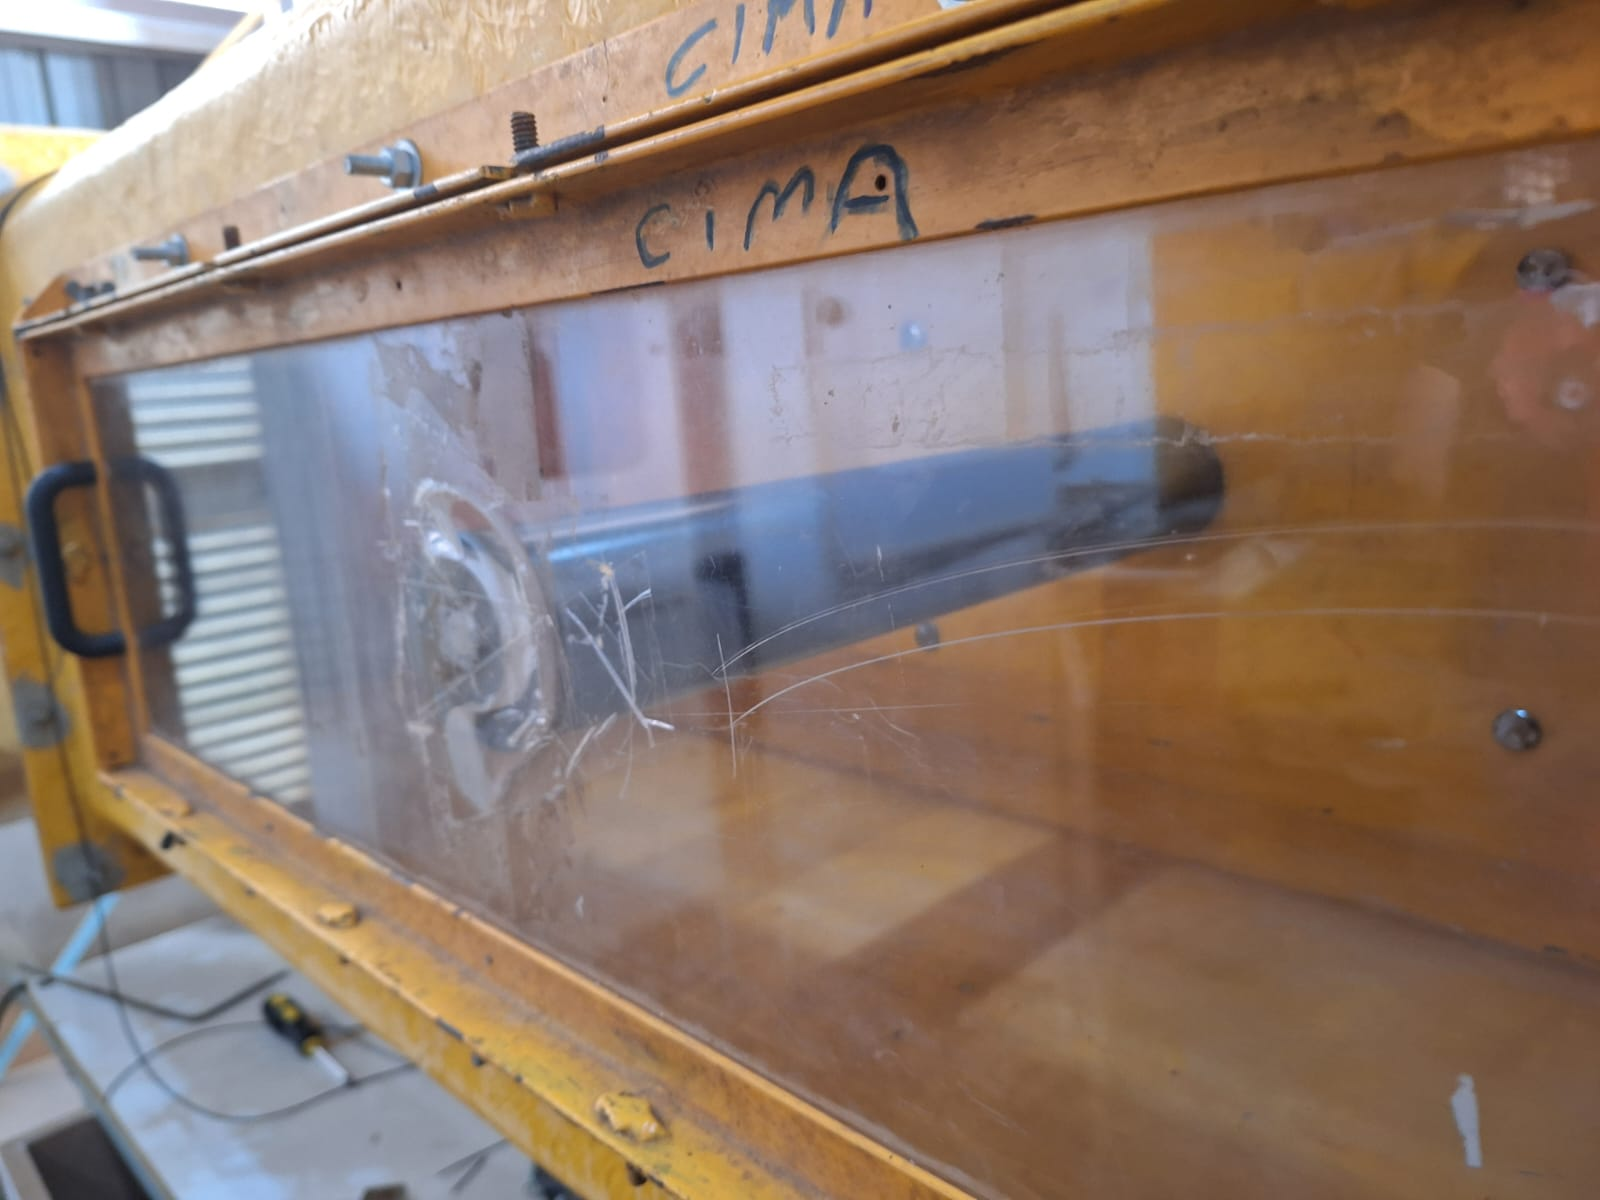
\includegraphics[width=\textwidth]{01.Parte1/Figuras/Cilindro - representação - vista em perspectiva.jpg}
        \caption{Montagem do cilindro no túnel de vento}
        \label{fig:Monta}
    \end{subfigure}
    
    \caption{Experimento de cilindro liso}
    \label{fig:dos_imagenes}
\end{figure}

Também foram calculados calculadas as seguintes variáveis e seus respectivos erros:
\begin{itemize}
    \item A densidade do ar
    \item Velocidade do escoamento livre
    \item Viscosidade dinâmica do ar
    \item Número de Reynolds
    \item Mach
\end{itemize}

Obtida das medidas de $C_p$, a Figura \ref{fig:Cp} mostra a comparação entre o coeficiente de pressão obtido no experimento e o coeficiente de pressão potencial (teórico).

Primeiramente, o método de cálculo dos erros de cada variável para uma função $z = f(x_{1}, x_{2}, \dots , x_{m})$ é:

\begin{equation}
   e_z =\sqrt{\sum_{i=1}^{m}\left ( \frac{\partial z}{\partial x_{i}} e_{x_{i}} \right )^{2} }  = \pm  \sqrt{\left ( \vec{\partial z}^{2}\cdot {\vec{e}}^{\ 2} \right )} 
\end{equation}

O produto escalar entre o quadrado dos vetores derivada parcial e erro, respectivamente. O primeiro é um vetor onde cada elemento $\vec{\partial z_{i}}$ corresponde à derivada parcial de $z$ em relação à variável $x_{i}$, e erro é um vetor onde cada elemento $\vec{e_{i}}$ corresponde ao erro da variável $x_{i}$.

As equações para o cálculo das variáveis apresentadas acima são mostradas a seguir:


\begin{subequations}
\label{eq:Variables_Cilindfro}
    \begin{multicols}{2}
        \begin{equation}
        \mu = \mu_0 \left( \frac{T}{T_{\text{ref}}} \right)^{\frac{3}{2}} \left( \frac{T_{\text{ref}} + S}{T + S} \right) = I T^{\frac{3}{2}}
        \end{equation}
        
        \begin{equation}
        \rho = \frac{P_{\text{sec}}}{287.058 \cdot T} + \frac{P_{\text{vap}}}{461.495 \cdot T} = W \frac{1}{T}
        \end{equation}
    
        \begin{equation}
        M = \frac{V_\infty}{\sqrt{\gamma R T}}
        \end{equation}
        \begin{equation}
        C_p = 1 - \frac{q}{q_{\infty}}= 1 - \frac{V}{V_{\infty}}
        \label{eq:Cp}
        \end{equation}
    
        \begin{equation}
        q_\infty = \frac{1}{2} \rho V_\infty^2 \Rightarrow V_\infty = \sqrt{\frac{2q_\infty}{\rho}}  
        \end{equation}
        
        \begin{equation}
        Re = \frac{\rho_{\infty} v_{\infty} c}{\mu} = \frac{\rho V_\infty D}{\mu}  
        \end{equation}
        
        \begin{equation}
        c = \sqrt{\gamma RT}
        \end{equation}
        
        \begin{equation}
        \bar{C}_{p} = 1-4 Sin^{2}\theta 
        \label{eq:potencial}
        \end{equation}
    \end{multicols}
\end{subequations}
Com isso, obtêm-se os vetores $\vec{\partial z_{i}}$ e $\vec{e_{i}}$ para cada equação, mostrados na Tabela \ref{tabla_1}. Cabe esclarecer que foram feitas as seguintes considerações:
\begin{enumerate}
    \item $ T + S = cte$
    \item $P_{\text{sec}} , P_{\text{vap}} \approx cte$ (durante o experimento)
    \item $\bar{C}_{p}$ refere-se ao coeficiente de pressão potencial
    \item $e_{q_{\infty}} = 0.1 ~ Pa$, equivalente ao erro do micromanômetro, tomado do manual.
    \item $e_q$ foi calculado com o desvio padrão dos dados coletados
    \item $e_{T} = e_{P_{atm}} = 0.1$ é o erro da Estação Meteorológica pelo manual
    \item $e_{D}$ é o erro da régua
    \item No cálculo do erro de Reynolds não é considerada a influência do $e_{\mu}$, devido ao fato de que esse erro é muito grande, porque na sua componente $\vec{   \partial }$,  $\mu^2$ é muito pequeno.
    \item Como cada $C_p$ tem seu erro, o erro da medição foi considerado como a média dos erros.


\end{enumerate}


\begin{table}[ht]
\centering
\caption{Resultados de cada variável}
\label{tabla_1}
\renewcommand{\arraystretch}{1.9} % Aumenta el tamaño vertical de las filas
\adjustbox{max width=\textwidth}{
\begin{tabular}{ccc|c|c}\toprule
       & \textbf{$\vec{   \partial }$}                                                                                                       & \textbf{$\vec{ e }$}                                & \textbf{Valor $\pm$ Error} & \textbf{Dimensões (SI)} \\ \toprule
$Re$   & $ \left(\frac{V_\infty D}{\mu},   \frac{\rho D}{\mu}, \frac{\rho V_\infty}{\mu}, \frac{-\rho V_\infty   D}{\mu^{2}}\right) $ & $e_{\rho}, e_{V_\infty}, e_{D},   e_{\mu}$ & $7.79 \cdot 10^{4} \pm 564$ &  \\
$\mu$  & $ \left(\frac{3 I   T^{\frac{1}{2}}}{2}\right) $                                                                             & $e_{T}$                                    & $1.86 \cdot 10^{-5} \pm 9.2 \cdot 10^{-9}$ & $\mathrm{kg \cdot m^{-1} \cdot s^{-1}}$ \\
$V_\infty$    & $ \left(\frac{-1}{2}\sqrt{\frac{2   q_\infty}{\rho^3}}, \frac{-1}{2}\sqrt{\frac{2}{\rho q_\infty}}\right) $                  & $e_{\rho}, e_{q_\infty}$                   & $18.10 \pm 6.1 \cdot 10^{-3}$ & $\mathrm{m \cdot s^{-1}}$ \\
$\rho$ & $ \left(\frac{-1}{T^2}\right) $                                                                                              & $e_{T}$                                    & $1.05 \pm 3.48 \cdot 10^{-4}$ & $\mathrm{kg \cdot m^{-3}}$ \\
$c$    & $   \left(\frac{1}{2}\sqrt{\frac{\gamma R}{T}}\right) $                                                                      & $e_{T}$                                    & $348.41 \pm 6.1 \cdot 10^{-2}$ & $\mathrm{m \cdot s^{-1}}$ \\
$C_p$  & $ \left(\frac{-q}{{q_\infty}^2},   \frac{1}{q_\infty}\right) $                                                               & $e_{q_\infty}, e_{q}$                      & $Cp \pm 0.42$ & \\
Ángulo & $1$                                                                                                                         & $e_{A}$                                  & Ángulo $\pm$ 0.5                & $^\circ$ \\ 
$M$    & $ \left(\frac{1}{c},   \frac{-V_\infty}{c^2}\right) $                                                                        & $e_{V_\infty}, e_{c}$                      & $5\cdot 10^{-2} \pm 1.9 \cdot 10^{-5}$ &  \\
$D$    & $1$                                                                                                                         & $e_{D}$                                    & $7.5\cdot 10^{-2} \pm 1 \cdot 10^{-3}$ & $\mathrm{m}$ \\
$P_{atm}$ & $1$                                                                                                                         & $e_{P_{atm}}$                             & $919.2\cdot 10^{2} \pm 0.1$ & $\mathrm{Pa}$ \\
$T$    & $1$                                                                                                                         & $e_{T}$                                    & $302.05 \pm 0.1$ & $\mathrm{K}$ \\
$RH$   & $1$                                                                                                                         & $e_{RH}$                                   & $55 \pm 0.1$ & $\%$ (relativa) \\ \bottomrule                    
\end{tabular}
}
\end{table}



Resolvendo o sistema de equações, obtêm-se os erros.














